\documentclass[12pt]{article}

\usepackage[a4paper,margin=1in]{geometry}
\usepackage{setspace}
\usepackage{graphicx}
\usepackage{booktabs}
\usepackage{array}
\usepackage{multirow}
\usepackage{amsmath}
\usepackage{url}
\usepackage[hidelinks]{hyperref}
\usepackage{caption}
\usepackage{subcaption}
\usepackage{longtable}

\doublespacing

\title{A Quality-Controlled Semi-Supervised Detection Framework\\for Cross-Domain Oil Palm\\Fresh Fruit Bunch Maturity Grading}

\author{
WU YUNING\textsuperscript{1,*}\\
\textsuperscript{1}School of Electrical Engineering and Artificial Intelligence,\\
Xiamen University Malaysia, Sepang, Malaysia\\
*Corresponding author: eee2309312@xmu.edu.my
}

\date{}

\begin{document}
\setlength{\emergencystretch}{3em}
\sloppy
\maketitle

\begin{abstract}
Automated oil palm fresh fruit bunch (FFB) maturity grading can support harvesting decisions, reduce manual subjectivity, and improve traceability in plantation operations. However, visual detection models trained on one image source often degrade when deployed across plantations, acquisition devices, lighting conditions, and dataset annotation protocols. This study presents a quality-controlled semi-supervised object detection framework for cross-domain oil palm FFB maturity grading. The framework starts from a YOLOv8n detector trained on a labeled source-domain video-frame dataset, introduces class-space harmonization across heterogeneous datasets, applies scene-disjoint evaluation to reduce frame-level leakage, and evaluates external-domain performance on a separate preprocessed FFB dataset with a four-class masked protocol. To improve robustness, the proposed pipeline combines class-balanced target-domain adaptation with strict pseudo-label filtering based on confidence, bounding-box geometry, edge-contact penalties, folder-level weak-label consistency, multi-view augmentation consistency, and class-wise dynamic confidence thresholds. Three random seeds were used for the main formal comparison. The source-only baseline achieved high scene-disjoint source-domain performance but collapsed on the locked external domain, with external mAP@0.5 of 0.0372 and mAP@0.5:0.95 of 0.0130, confirming severe domain shift. A class-balanced target-domain adaptation model improved external mAP@0.5 to 0.6973 and mAP@0.5:0.95 to 0.4758. A precision-first strict SSOD model achieved calibrated external mAP@0.5 of 0.7240, mAP@0.5:0.95 of 0.4863, precision of 0.8753, recall of 0.5364, and F1-score of 0.6321. A third-domain zero-shot image-level evaluation further indicated improved transfer relative to the source-only baseline. The results show that external-domain adaptation and quality-controlled pseudo-label selection can produce a more conservative and field-oriented FFB maturity detector, although under-ripe fruit bunches remain the main error source.
\end{abstract}

\textbf{Keywords:} oil palm; fresh fruit bunch; maturity grading; object detection; semi-supervised learning; YOLOv8; domain adaptation; agricultural engineering

\section{Introduction}

Oil palm fresh fruit bunch (FFB) maturity grading is a key operational step in plantation management and palm oil production. Harvesting unripe bunches reduces oil extraction efficiency, whereas delayed harvesting can increase overripe bunches, loose fruit loss, and quality degradation. In practice, FFB maturity is often judged manually from color, texture, and fruit detachment cues. Manual grading is inexpensive and flexible, but it is also subjective, labor-intensive, and sensitive to worker experience, illumination, occlusion, and the mixture of bunches in piles or field scenes \cite{suharjito2023dataset,omar2024outdoor}.

Computer vision has therefore been widely explored for agricultural quality assessment, fruit detection, and maturity grading \cite{kamilaris2018survey,bargoti2017fruit}. Modern object detectors, especially one-stage detectors in the YOLO family, are attractive for field applications because they provide a practical compromise between accuracy and inference speed \cite{redmon2016yolo,jocher2023yolov8}. For oil palm FFB maturity detection, a detector must localize bunches and distinguish visually similar maturity categories such as unripe, under-ripe, ripe, and overripe. Previous oil palm studies have shown the feasibility of deep learning and YOLO-based approaches for FFB ripeness classification or detection \cite{suharjito2021mobile,lai2022yolov4,mansour2022object}. However, this task remains more difficult than simple fruit presence detection because the decision boundary depends on fine color transitions, fruit surface texture, shadows, and camera exposure.

A major limitation of many agricultural detection studies is that the reported performance is often measured on random splits or same-source test sets. For video-frame datasets, random splitting can overestimate performance because adjacent frames from the same video, pile, lighting condition, or acquisition session may appear in both training and testing subsets. A model may therefore learn scene-specific appearance rather than robust maturity cues. When deployed on another dataset or plantation scene, performance can drop sharply. This issue is especially important for oil palm FFB maturity grading because available datasets are heterogeneous: some are collected from videos of fruit bunch piles \cite{suharjito2023dataset}, others from outdoor plantation scenes \cite{omar2024outdoor}, and others are preprocessed into class folders or weakly labeled subsets.

This study reframes oil palm FFB maturity detection as a cross-domain agricultural engineering problem rather than a single-dataset YOLO training task. The central hypothesis is that a source-domain detector trained on video-frame data can perform well in-domain but fail on an external domain, and that this failure can be mitigated by combining target-domain adaptation with quality-controlled semi-supervised object detection (SSOD). The proposed framework is designed to be conservative: pseudo-labels are not accepted solely from high detector confidence, but must also satisfy geometry constraints, edge-contact penalties, weak class-folder consistency, multi-view augmentation consistency, and class-wise dynamic thresholds.

The main contributions of this work are as follows. First, a strict evaluation protocol is introduced for oil palm FFB maturity detection, including source-domain scene-disjoint evaluation, locked external-domain testing, and four-class masked evaluation when the target dataset lacks empty and overripe categories. Second, a class-space harmonization strategy is used to integrate source and external datasets with inconsistent maturity labels while avoiding invalid class penalties in missing-class datasets. Third, a quality-controlled SSOD pipeline is implemented to filter pseudo-labeled images under multi-view consistency and class-balanced selection. Fourth, formal three-seed experiments are reported for a source-only baseline, a class-balanced target-domain adaptation baseline, and a precision-first strict SSOD model. The results are interpreted conservatively: the large gain from source-only to target-adapted models is evidence of domain adaptation, not zero-shot generalization.

\section{Materials and Methods}

\subsection{Datasets and Class Harmonization}

The experimental pipeline used three dataset roles, summarized in Table~\ref{tab:dataset_roles}. The first was a labeled source-domain oil palm FFB dataset based mainly on ScienceDB/OILPALM-style video-frame imagery \cite{suharjito2023dataset}. This dataset was used to train the source-only supervised baseline and to construct a scene-disjoint split. The second was an external-domain preprocessed FFB dataset, which was used as the main target-domain dataset for cross-domain evaluation and adaptation. The third was an outdoor oil palm ripeness dataset used only for exploratory third-domain zero-shot image-level evaluation \cite{omar2024outdoor}.

The unified class scheme contained six maturity or condition classes (Table~\ref{tab:class_scheme}):
\[
\mathcal{C}=\{\text{abnormal},\text{empty},\text{overripe},\text{ripe},\text{under\_ripe},\text{unripe}\}.
\]
Because the external preprocessed FFB dataset did not contain empty and overripe classes, the external evaluation was performed under a masked four-class protocol:
\[
\mathcal{C}_{ext}=\{\text{abnormal},\text{ripe},\text{under\_ripe},\text{unripe}\}.
\]
Empty and overripe predictions were ignored for this external protocol. This prevents the model from being penalized for classes that were absent from the external dataset and allows a fairer comparison across heterogeneous label spaces.

To reduce overly optimistic evaluation caused by adjacent video frames, the source-domain data were not used only under a random split. A video- or scene-disjoint split was constructed based on filename prefixes or inferred video identifiers. Frames from the same scene group were assigned to the same split. The official or original source-domain split was retained only as an in-domain reference and was not used as the main conclusion.

\subsection{Model Stages}

Four model stages were considered during development, but the formal manuscript focuses on three main stages.

\textbf{Source-only YOLOv8n baseline.} The first model was a YOLOv8n detector initialized from COCO-pretrained weights and trained only on the source-domain labeled dataset. This model represents the common supervised baseline and is used to quantify the cross-domain collapse when evaluated on the external FFB dataset.

\textbf{Class-balanced target-domain adaptation model.} The second model, denoted Model2 Balanced, used source-domain data together with a class-balanced supervised subset of the external-domain training data. This model is not a zero-shot model; it represents a practical target-domain adaptation baseline. It was included because comparing the final system only against the weak source-only baseline would exaggerate the improvement.

\textbf{Precision-first strict SSOD model.} The third model applied quality-controlled pseudo-label self-training on top of the adapted teacher. It was designed for high-precision deployment, where false positives in maturity grading are operationally costly. The SSOD stage used multi-view consistency, quality scoring, dynamic class-wise thresholds, and class-balanced pseudo-label acceptance.

\subsection{Pseudo-Label Generation with Multi-View Consistency}

For each candidate unlabeled or weakly labeled image, the teacher detector generated predictions on the original image and on augmented views. Augmentations included brightness and contrast jitter, horizontal or vertical flips, small rotations, and crop-like perturbations. Predictions from augmented views were mapped back to the original image coordinate system. A pseudo-label candidate was accepted only when boxes from the original and augmented views agreed in class and localization. The localization consistency was measured using intersection-over-union (IoU), and inconsistent predictions were rejected.

This design follows the general principle of consistency regularization in semi-supervised learning: a reliable object prediction should remain stable under label-preserving image transformations \cite{tarvainen2017mean,sohn2020fixmatch}. In this work, consistency was used as a filtering criterion rather than a fully online teacher-student loss, making the method easier to reproduce with standard YOLOv8 training tools. The approach is related to pseudo-label and consistency-based SSOD methods \cite{sohn2020stac,liu2021unbiased,xu2021softteacher,li2022pseco}, but it is implemented as an offline quality-control layer for an agricultural engineering workflow.

\subsection{Pseudo-Label Quality Score}

Each predicted bounding box was assigned a composite quality score:
\[
Q = w_c Q_c + w_g Q_g + w_e Q_e + w_f Q_f + w_m Q_m ,
\]
where \(Q_c\) is detector confidence, \(Q_g\) is a geometry score, \(Q_e\) is an edge-contact score, \(Q_f\) is weak folder-level class consistency, \(Q_m\) is multi-view consistency, and \(w_c,\ldots,w_m\) are non-negative weights. The geometry score penalized boxes with implausible normalized area or aspect ratio. The edge score penalized boxes touching image boundaries, because such boxes often represent incomplete bunches or truncated detections. The folder-consistency score used class-folder information only as an image-level weak prior, not as bounding-box ground truth. This distinction is important: the method is weak-label-guided SSOD rather than purely unlabeled SSOD.

Pseudo-labels were filtered by both a global quality threshold and class-wise confidence thresholds. Images were then selected under a class-balanced quota so that abundant easy classes did not dominate the pseudo-labeled training set.

\subsection{Dynamic Class-Wise Thresholds}

Class-wise thresholds were updated using validation statistics. Classes with weaker validation performance or higher confusion risk were assigned stricter confidence thresholds, while easier classes could use lower thresholds. This mechanism was intended to reduce noisy pseudo-labels for visually difficult categories, especially under-ripe and unripe bunches, which often share color and texture cues.

For deployment-style reporting, class-wise calibrated thresholds were also selected for a high-precision operating point. This is appropriate for maturity grading scenarios where a conservative detector may be preferred over a detector that maximizes recall at the cost of many false positives.

\subsection{Training and Evaluation Protocol}

All YOLOv8 training was performed using the Ultralytics Python API with Windows-compatible settings, including \texttt{workers=0}. The input resolution for formal external evaluation was 640 pixels. Three random seeds were used for the formal comparison: 42, 2026, and 3407.

The following evaluation layers were used:

\begin{enumerate}
    \item \textbf{Scene-disjoint source-domain test}: evaluates source-domain generalization across held-out video or scene groups.
    \item \textbf{Locked external-domain test}: evaluates cross-domain detection on the preprocessed FFB dataset using the four-class masked protocol.
    \item \textbf{Calibration evaluation}: reports a high-precision external operating point with calibrated class-wise thresholds.
    \item \textbf{Third-domain zero-shot evaluation}: evaluates image-level class prediction on an outdoor oil palm dataset that was not used for training.
\end{enumerate}

The primary detection metrics were precision, recall, F1-score, mAP@0.5, and mAP@0.5:0.95. The third-domain experiment was reported separately as image-level top-1 accuracy and macro F1-score, and should not be compared directly with detection mAP.

\section{Results}

\subsection{Domain Shift from Source-Only Training}

The source-only YOLOv8n model achieved scene-disjoint source-domain mAP@0.5 of 0.5917 and mAP@0.5:0.95 of 0.5018 across three seeds (Table~\ref{tab:formal_results}). However, when evaluated on the locked external preprocessed FFB dataset, performance dropped to mAP@0.5 of 0.0372 and mAP@0.5:0.95 of 0.0130. This confirms severe cross-domain degradation. Therefore, the source-only result was used as evidence of domain shift rather than as the main baseline for claiming method improvement.

The class-balanced target-domain adaptation model substantially improved external-domain performance, reaching external mAP@0.5 of 0.6973 and mAP@0.5:0.95 of 0.4758. This result demonstrates that using the external-domain training portion for adaptation can recover target-domain detection performance. It does not demonstrate zero-shot generalization, because external-domain data were used during training.

\subsection{Strict SSOD and High-Precision Calibration}

The precision-first strict SSOD model achieved scene-disjoint mAP@0.5 of 0.6373 and mAP@0.5:0.95 of 0.5408. Under calibrated external-domain evaluation, it achieved mAP@0.5 of 0.7240, mAP@0.5:0.95 of 0.4863, precision of 0.8753, recall of 0.5364, and F1-score of 0.6321 (Table~\ref{tab:strict_ssod}; Fig.~\ref{fig:external_map}). Compared with the class-balanced adaptation baseline, strict SSOD mainly improved the high-precision operating point rather than producing a large headline mAP improvement. The calibration curve in Fig.~\ref{fig:calibration} illustrates this precision-recall trade-off.

This behavior is consistent with the design of the method. Strict pseudo-label filtering and high class-wise thresholds reject uncertain detections, reducing false positives but also reducing recall. For field deployment, this may be desirable when the cost of incorrect maturity grading is high. For exhaustive counting or harvest-yield estimation, the lower recall would require further optimization.

\subsection{Third-Domain Zero-Shot Image-Level Evaluation}

On the outdoor third-domain dataset, the source-only model achieved image-level top-1 accuracy of 0.4632 and macro F1-score of 0.3480 (Table~\ref{tab:third_domain}). Model2 Balanced improved top-1 accuracy to 0.6000 and macro F1-score to 0.4383. Strict SSOD further improved top-1 accuracy to 0.6351 but had lower macro F1-score of 0.4048. This indicates that strict SSOD improved overall image-level correctness but did not uniformly improve all classes. The third-domain dataset was relatively small, with 95 images per seed in the evaluation, so these results should be treated as exploratory evidence rather than definitive proof of generalization.

\subsection{Under-Ripe Error Analysis}

Under-ripe FFB remained the most difficult category. In the seed-2026 locked external analysis, Model2 Balanced achieved under-ripe AP@0.5 of 0.7528 and AP@0.5:0.95 of 0.5352, with 24 false-negative under-ripe cases and 8 misclassified under-ripe cases (Table~\ref{tab:under_ripe}). Strict SSOD achieved lower under-ripe AP@0.5 of 0.6657 and AP@0.5:0.95 of 0.4918, with 48 false negatives and 5 misclassifications. This suggests that strict filtering reduced some class confusion but also made the detector more conservative for under-ripe bunches. The confusion matrices in Fig.~\ref{fig:confusion_model2} and Fig.~\ref{fig:confusion_strict} show the corresponding external-domain class-level behaviour.

The under-ripe limitation is technically plausible. Under-ripe bunches lie between unripe and ripe in the maturity continuum and can be visually ambiguous under different lighting conditions. Future improvements should focus on ordinal maturity modeling, targeted under-ripe positive sampling, and richer color-calibrated field data rather than only increasing the amount of pseudo-labeled data.

\subsection{Engineering Interpretation}

The results support three engineering interpretations. First, random or same-source evaluation is insufficient for oil palm FFB maturity detection. The large gap between source-domain scene-disjoint performance and locked external-domain performance shows that a detector trained on one data source may not generalize to another without adaptation. This is especially important for video-frame datasets, where adjacent frames can produce optimistic random-split metrics.

Second, target-domain adaptation is the dominant source of external-domain recovery. The improvement from source-only external mAP@0.5 of 0.0372 to Model2 Balanced external mAP@0.5 of 0.6973 should not be presented as a pure SSOD gain. It reflects the transition from source-only training to target-domain adaptation using the external training portion. This interpretation is important for scientific validity and for avoiding inflated claims.

Third, strict SSOD contributes mainly to conservative deployment behavior. The precision-first model achieved high calibrated precision of 0.8753, but recall was 0.5364. This trade-off is relevant in agricultural engineering practice. If the system is used to flag high-confidence maturity classes for quality control, high precision is valuable. If the system is used to count all bunches or automate complete grading, additional recall-focused improvements are necessary.

The proposed framework has several limitations. The external preprocessed FFB dataset lacks empty and overripe categories, requiring masked evaluation. Although this is methodologically necessary, it means the reported external-domain result does not cover the full six-class maturity scheme. The third-domain outdoor dataset was used only for image-level evaluation and had limited class balance, so it cannot replace a large object-detection external test set. Finally, the SSOD stage used offline pseudo-label filtering rather than a fully online exponential moving average teacher-student training loop. This choice improves reproducibility and engineering simplicity but may limit the maximum performance gain.

\section{Conclusions}

This study developed a quality-controlled semi-supervised YOLOv8 framework for cross-domain oil palm FFB maturity detection. The framework combines class-space harmonization, scene-disjoint evaluation, locked external-domain testing, class-balanced target-domain adaptation, multi-view pseudo-label consistency, composite pseudo-label quality scoring, dynamic class-wise thresholds, and high-precision calibration.

The experiments show that source-only training on video-frame data can fail severely on an external FFB dataset, confirming strong domain shift. Class-balanced target-domain adaptation substantially improves external detection performance. Strict SSOD provides a more conservative high-precision operating point, achieving calibrated external precision of 0.8753 with mAP@0.5 of 0.7240, although recall remains limited. Under-ripe detection remains the main bottleneck because it is visually close to neighboring maturity stages.

For practical deployment, the proposed framework is most suitable as a conservative decision-support system for FFB maturity grading rather than a complete replacement for human inspection. Future work should expand third-domain detection data, add ordinal maturity constraints, collect more under-ripe boundary cases, and evaluate the system on continuous field video streams.

\section*{Data Availability Statement}

The source and external datasets used in this study were derived from publicly available or locally prepared oil palm FFB datasets. The manuscript repository contains the class-space definition, selected formal evaluation outputs, and the code needed to reproduce the preparation and evaluation protocol. Raw images and trained weights are not redistributed in the repository because their redistribution depends on the licenses and access conditions of the original datasets. Processed split manifests and additional evaluation outputs can be shared by the corresponding author upon reasonable request where permitted by the original data licenses.

\section*{Code Availability Statement}

The implementation was developed in Python using the Ultralytics YOLOv8 API. The pipeline includes dataset preparation, scene-disjoint splitting, duplicate checking, pseudo-label generation, quality scoring, class-wise threshold calibration, and structured JSON/CSV reporting. The public repository is available at \url{https://github.com/yuningwuyn-lgtm/oil-palm-ffb-ssod}. The repository contains source code, configuration templates, manuscript files, and selected evaluation reports; raw third-party datasets and trained weights are excluded because their redistribution depends on the licenses and access conditions of the original data providers.

\section*{Conflict of Interest}

The author declares no conflict of interest.

\section*{Funding}

This research received no external funding.

\section*{Acknowledgements}

The author thanks the maintainers of the public oil palm FFB datasets and the open-source computer vision libraries used in this work.

\section*{CRediT Authorship Contribution}

WU YUNING: conceptualization, methodology, software, validation, formal analysis, data curation, writing-original draft preparation, visualization, and project administration.

\section*{Supporting Agencies}

No external supporting agency was involved in this study.

\begin{thebibliography}{99}

\bibitem{suharjito2023dataset}
Suharjito, F. A. Junior, Y. P. Koeswandy, Debi, P. W. Nurhayati, M. Asrol, and Marimin, ``Annotated datasets of oil palm fruit bunch piles for ripeness grading using deep learning,'' \textit{Scientific Data}, vol. 10, article 72, 2023.

\bibitem{omar2024outdoor}
Z. Omar, A. P. P. Abdul Majeed, M. Rosbi, S. A. Ghazalli, and H. Selamat, ``Outdoor oil palm fruit ripeness dataset,'' \textit{Data in Brief}, vol. 55, article 110667, 2024.

\bibitem{kamilaris2018survey}
A. Kamilaris and F. X. Prenafeta-Boldu, ``Deep learning in agriculture: A survey,'' \textit{Computers and Electronics in Agriculture}, vol. 147, pp. 70--90, 2018.

\bibitem{bargoti2017fruit}
S. Bargoti and J. Underwood, ``Deep fruit detection in orchards,'' in \textit{IEEE International Conference on Robotics and Automation}, 2017, pp. 3626--3633.

\bibitem{redmon2016yolo}
J. Redmon, S. Divvala, R. Girshick, and A. Farhadi, ``You only look once: Unified, real-time object detection,'' in \textit{Proceedings of the IEEE Conference on Computer Vision and Pattern Recognition}, 2016, pp. 779--788.

\bibitem{jocher2023yolov8}
G. Jocher, A. Chaurasia, and J. Qiu, ``Ultralytics YOLOv8,'' 2023. [Online]. Available: \url{https://github.com/ultralytics/ultralytics}

\bibitem{suharjito2021mobile}
Suharjito, G. N. Elwirehardja, and J. S. Prayoga, ``Oil palm fresh fruit bunch ripeness classification on mobile devices using deep learning approaches,'' \textit{Computers and Electronics in Agriculture}, vol. 188, article 106359, 2021.

\bibitem{lai2022yolov4}
J. W. Lai, H. R. Ramli, L. I. Ismail, and W. Z. W. Hasan, ``Real-time detection of ripe oil palm fresh fruit bunch based on YOLOv4,'' \textit{IEEE Access}, vol. 10, pp. 95763--95770, 2022.

\bibitem{mansour2022object}
M. Y. M. A. Mansour, K. D. Dambul, and K. Y. Choo, ``Object detection algorithms for ripeness classification of oil palm fresh fruit bunch,'' \textit{International Journal of Technology}, vol. 13, no. 6, pp. 1326--1335, 2022.

\bibitem{tarvainen2017mean}
A. Tarvainen and H. Valpola, ``Mean teachers are better role models: Weight-averaged consistency targets improve semi-supervised deep learning results,'' in \textit{Advances in Neural Information Processing Systems}, 2017.

\bibitem{sohn2020fixmatch}
K. Sohn et al., ``FixMatch: Simplifying semi-supervised learning with consistency and confidence,'' in \textit{Advances in Neural Information Processing Systems}, 2020.

\bibitem{sohn2020stac}
K. Sohn et al., ``A simple semi-supervised learning framework for object detection,'' \textit{arXiv preprint arXiv:2005.04757}, 2020.

\bibitem{liu2021unbiased}
Y.-C. Liu et al., ``Unbiased teacher for semi-supervised object detection,'' in \textit{International Conference on Learning Representations}, 2021.

\bibitem{xu2021softteacher}
M. Xu et al., ``End-to-end semi-supervised object detection with soft teacher,'' in \textit{Proceedings of the IEEE/CVF International Conference on Computer Vision}, 2021.

\bibitem{li2022pseco}
J. Li et al., ``PseCo: Pseudo labeling and consistency training for semi-supervised object detection,'' in \textit{European Conference on Computer Vision}, 2022.

\end{thebibliography}

\clearpage
\section*{Tables}

\begin{table}[h]
\centering
\caption{Dataset roles used in the cross-domain evaluation protocol.}
\label{tab:dataset_roles}
\resizebox{\textwidth}{!}{%
\begin{tabular}{llll}
\toprule
Dataset role & Main use & Supervision type & Evaluation note \\
\midrule
Source-domain ScienceDB/OILPALM-style video frames & Source training and scene-disjoint testing & Bounding-box labels & Used to quantify in-domain and video/scene generalization \\
External preprocessed FFB & Target-domain adaptation and locked external testing & Four-class detection protocol & Empty and overripe ignored during masked external evaluation \\
Outdoor oil palm ripeness dataset & Third-domain exploratory testing & Image-level class labels & Used only for zero-shot image-level transfer analysis \\
Unlabeled or weakly labeled images & Pseudo-label self-training & Folder-level weak prior or unlabeled & Filtered by quality score and multi-view consistency \\
\bottomrule
\end{tabular}}
\end{table}

\begin{table}[h]
\centering
\caption{Unified class scheme and external-domain masked evaluation setting.}
\label{tab:class_scheme}
\begin{tabular}{lll}
\toprule
Class ID & Unified class & Used in external masked evaluation \\
\midrule
0 & abnormal & Yes \\
1 & empty & Ignored \\
2 & overripe & Ignored \\
3 & ripe & Yes \\
4 & under\_ripe & Yes \\
5 & unripe & Yes \\
\bottomrule
\end{tabular}
\end{table}

\begin{table}[h]
\centering
\caption{Formal three-seed detection results. Values are mean $\pm$ standard deviation.}
\label{tab:formal_results}
\resizebox{\textwidth}{!}{%
\begin{tabular}{lccccccc}
\toprule
Model & Scene mAP@0.5 & Scene mAP@0.5:0.95 & External mAP@0.5 & External mAP@0.5:0.95 & External precision & External recall & External F1 \\
\midrule
Source-only YOLOv8n & $0.5917 \pm 0.0339$ & $0.5018 \pm 0.0343$ & $0.0372 \pm 0.0221$ & $0.0130 \pm 0.0075$ & $0.1640 \pm 0.0747$ & $0.0933 \pm 0.0530$ & $0.0735 \pm 0.0308$ \\
Model2 Balanced & $0.6459 \pm 0.0190$ & $0.5484 \pm 0.0149$ & $0.6973 \pm 0.0298$ & $0.4758 \pm 0.0175$ & $0.6126 \pm 0.0323$ & $0.7527 \pm 0.0121$ & $0.6442 \pm 0.0332$ \\
Stage-1 SSOD teacher & $0.6141 \pm 0.0340$ & $0.5125 \pm 0.0183$ & $0.6619 \pm 0.0283$ & $0.4462 \pm 0.0309$ & $0.6163 \pm 0.0468$ & $0.7411 \pm 0.0473$ & $0.6390 \pm 0.0174$ \\
Stage-2 refined & $0.5878 \pm 0.0436$ & $0.4900 \pm 0.0395$ & $0.6754 \pm 0.0430$ & $0.4645 \pm 0.0331$ & $0.6294 \pm 0.0402$ & $0.7427 \pm 0.0338$ & $0.6743 \pm 0.0386$ \\
\bottomrule
\end{tabular}}
\end{table}

\begin{table}[h]
\centering
\caption{Precision-first strict SSOD calibrated external-domain results across three seeds.}
\label{tab:strict_ssod}
\begin{tabular}{lcc}
\toprule
Metric & Mean & Standard deviation \\
\midrule
Scene-disjoint mAP@0.5 & 0.6373 & 0.0286 \\
Scene-disjoint mAP@0.5:0.95 & 0.5408 & 0.0276 \\
Calibrated external mAP@0.5 & 0.7240 & 0.0072 \\
Calibrated external mAP@0.5:0.95 & 0.4863 & 0.0038 \\
Calibrated external precision & 0.8753 & 0.0116 \\
Calibrated external recall & 0.5364 & 0.0232 \\
Calibrated external F1-score & 0.6321 & 0.0294 \\
\bottomrule
\end{tabular}
\end{table}

\begin{table}[h]
\centering
\caption{Third-domain zero-shot image-level evaluation. Detection mAP is not reported for this dataset because the protocol is image-level.}
\label{tab:third_domain}
\resizebox{\textwidth}{!}{%
\begin{tabular}{lcccc}
\toprule
Model & Top-1 accuracy & Macro precision & Macro recall & Macro F1 \\
\midrule
Source-only YOLOv8n & $0.4632 \pm 0.0459$ & $0.3936 \pm 0.0690$ & $0.4078 \pm 0.0974$ & $0.3480 \pm 0.0565$ \\
Model2 Balanced & $0.6000 \pm 0.0380$ & $0.4804 \pm 0.1305$ & $0.4585 \pm 0.0905$ & $0.4383 \pm 0.1035$ \\
Strict SSOD & $0.6351 \pm 0.0338$ & $0.4015 \pm 0.0436$ & $0.4451 \pm 0.0275$ & $0.4048 \pm 0.0336$ \\
\bottomrule
\end{tabular}}
\end{table}

\begin{table}[h]
\centering
\caption{Seed-2026 under-ripe class analysis on the locked external dataset.}
\label{tab:under_ripe}
\resizebox{\textwidth}{!}{%
\begin{tabular}{lcccc}
\toprule
Model & Under-ripe AP@0.5 & Under-ripe AP@0.5:0.95 & False negatives & Misclassified cases \\
\midrule
Model2 Balanced & 0.7528 & 0.5352 & 24 & 8 \\
Strict SSOD & 0.6657 & 0.4918 & 48 & 5 \\
\bottomrule
\end{tabular}}
\end{table}

\clearpage
\section*{Figures}

\begin{figure}[h]
\centering
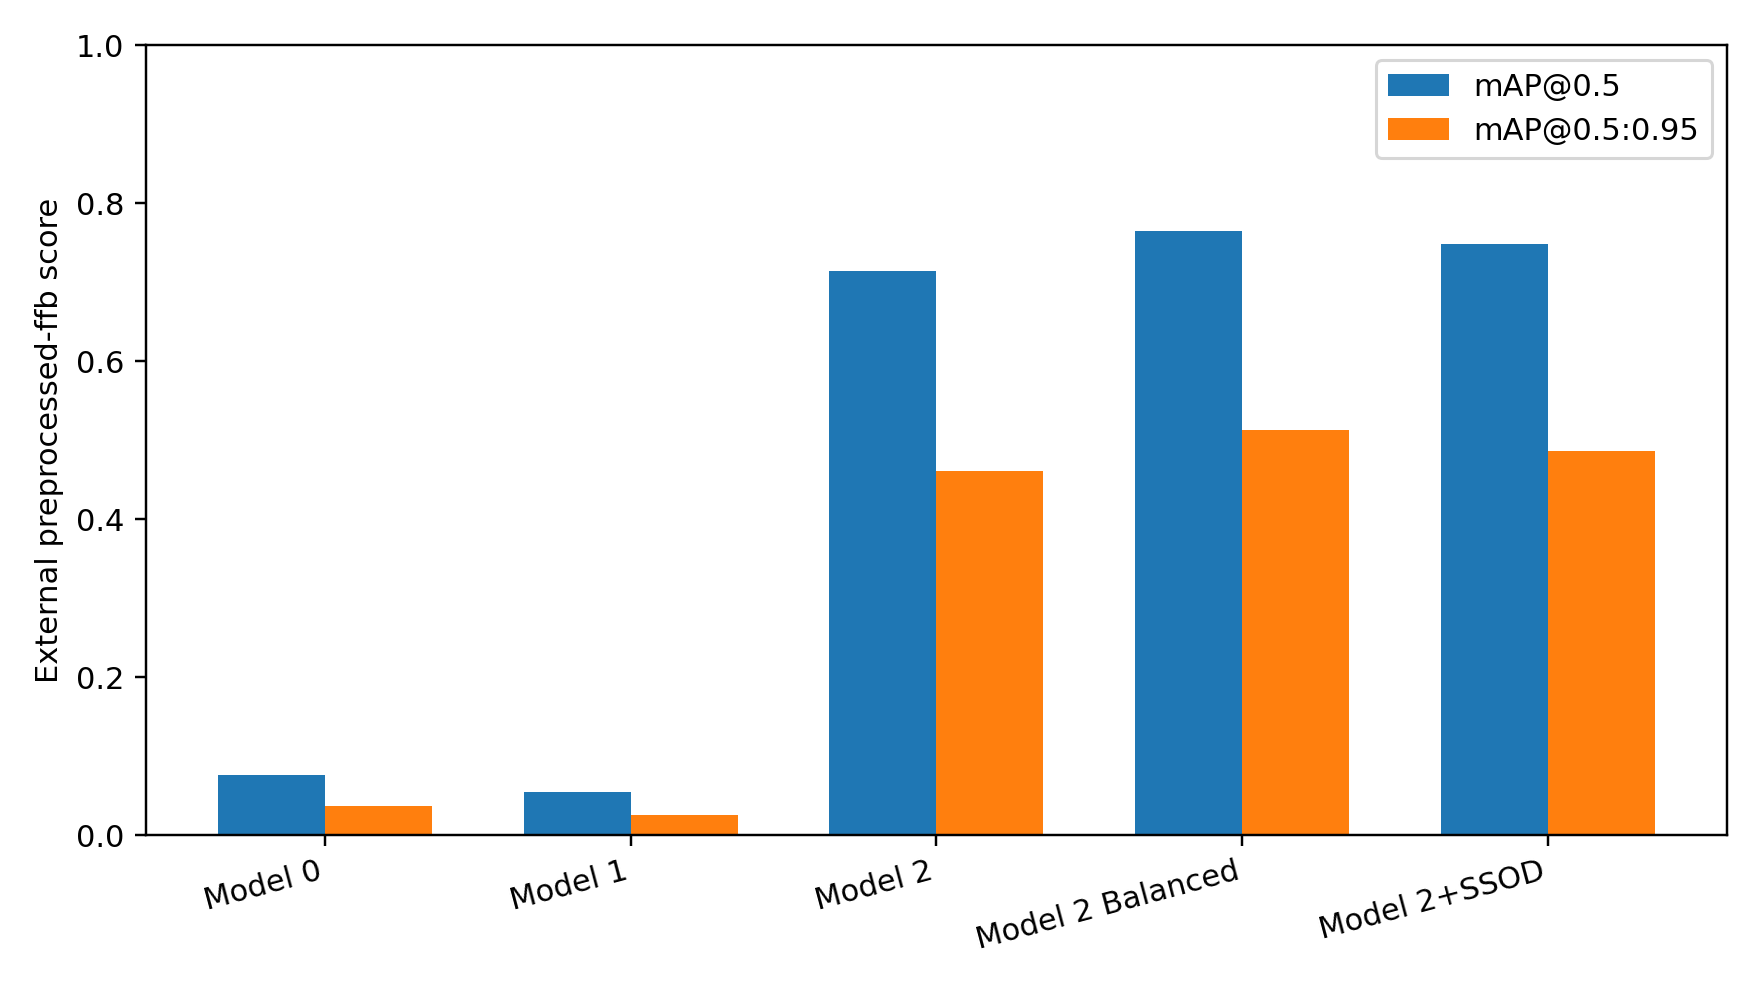
\includegraphics[width=0.85\textwidth]{figures/fig_external_map.png}
\caption{External-domain model comparison plot generated from the project reporting pipeline.}
\label{fig:external_map}
\end{figure}

\begin{figure}[h]
\centering
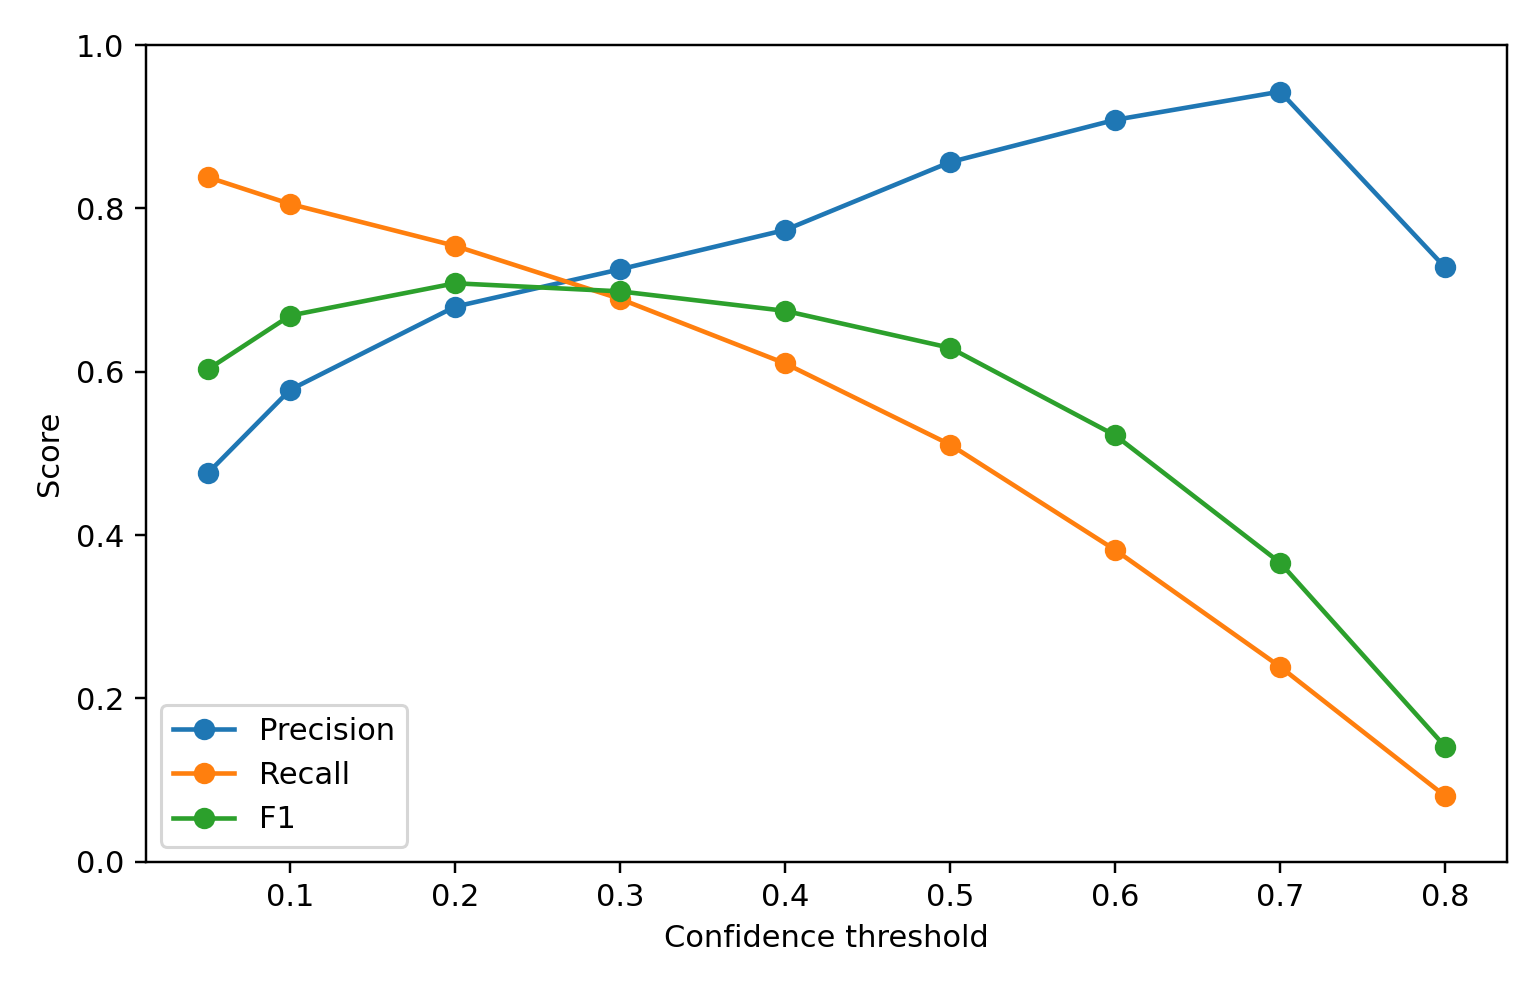
\includegraphics[width=0.85\textwidth]{figures/fig_calibration_curve.png}
\caption{External-domain calibration curve used to select high-precision operating points.}
\label{fig:calibration}
\end{figure}

\begin{figure}[h]
\centering
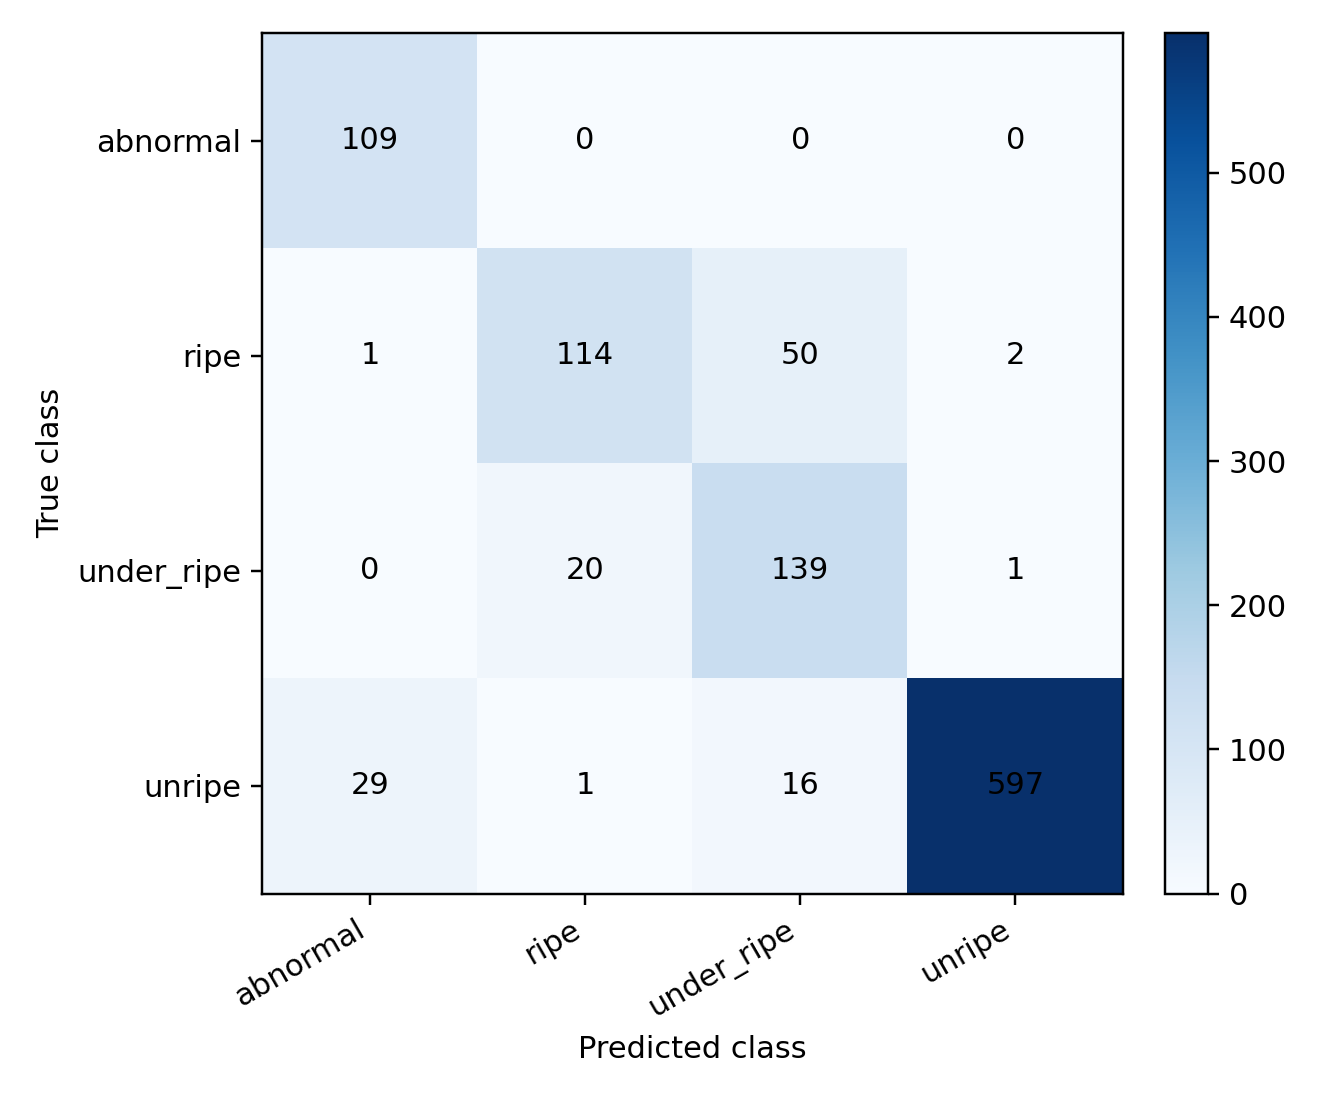
\includegraphics[width=0.75\textwidth]{figures/fig_confusion_matrix.png}
\caption{External-domain confusion matrix for the class-balanced target-domain adaptation model.}
\label{fig:confusion_model2}
\end{figure}

\begin{figure}[h]
\centering
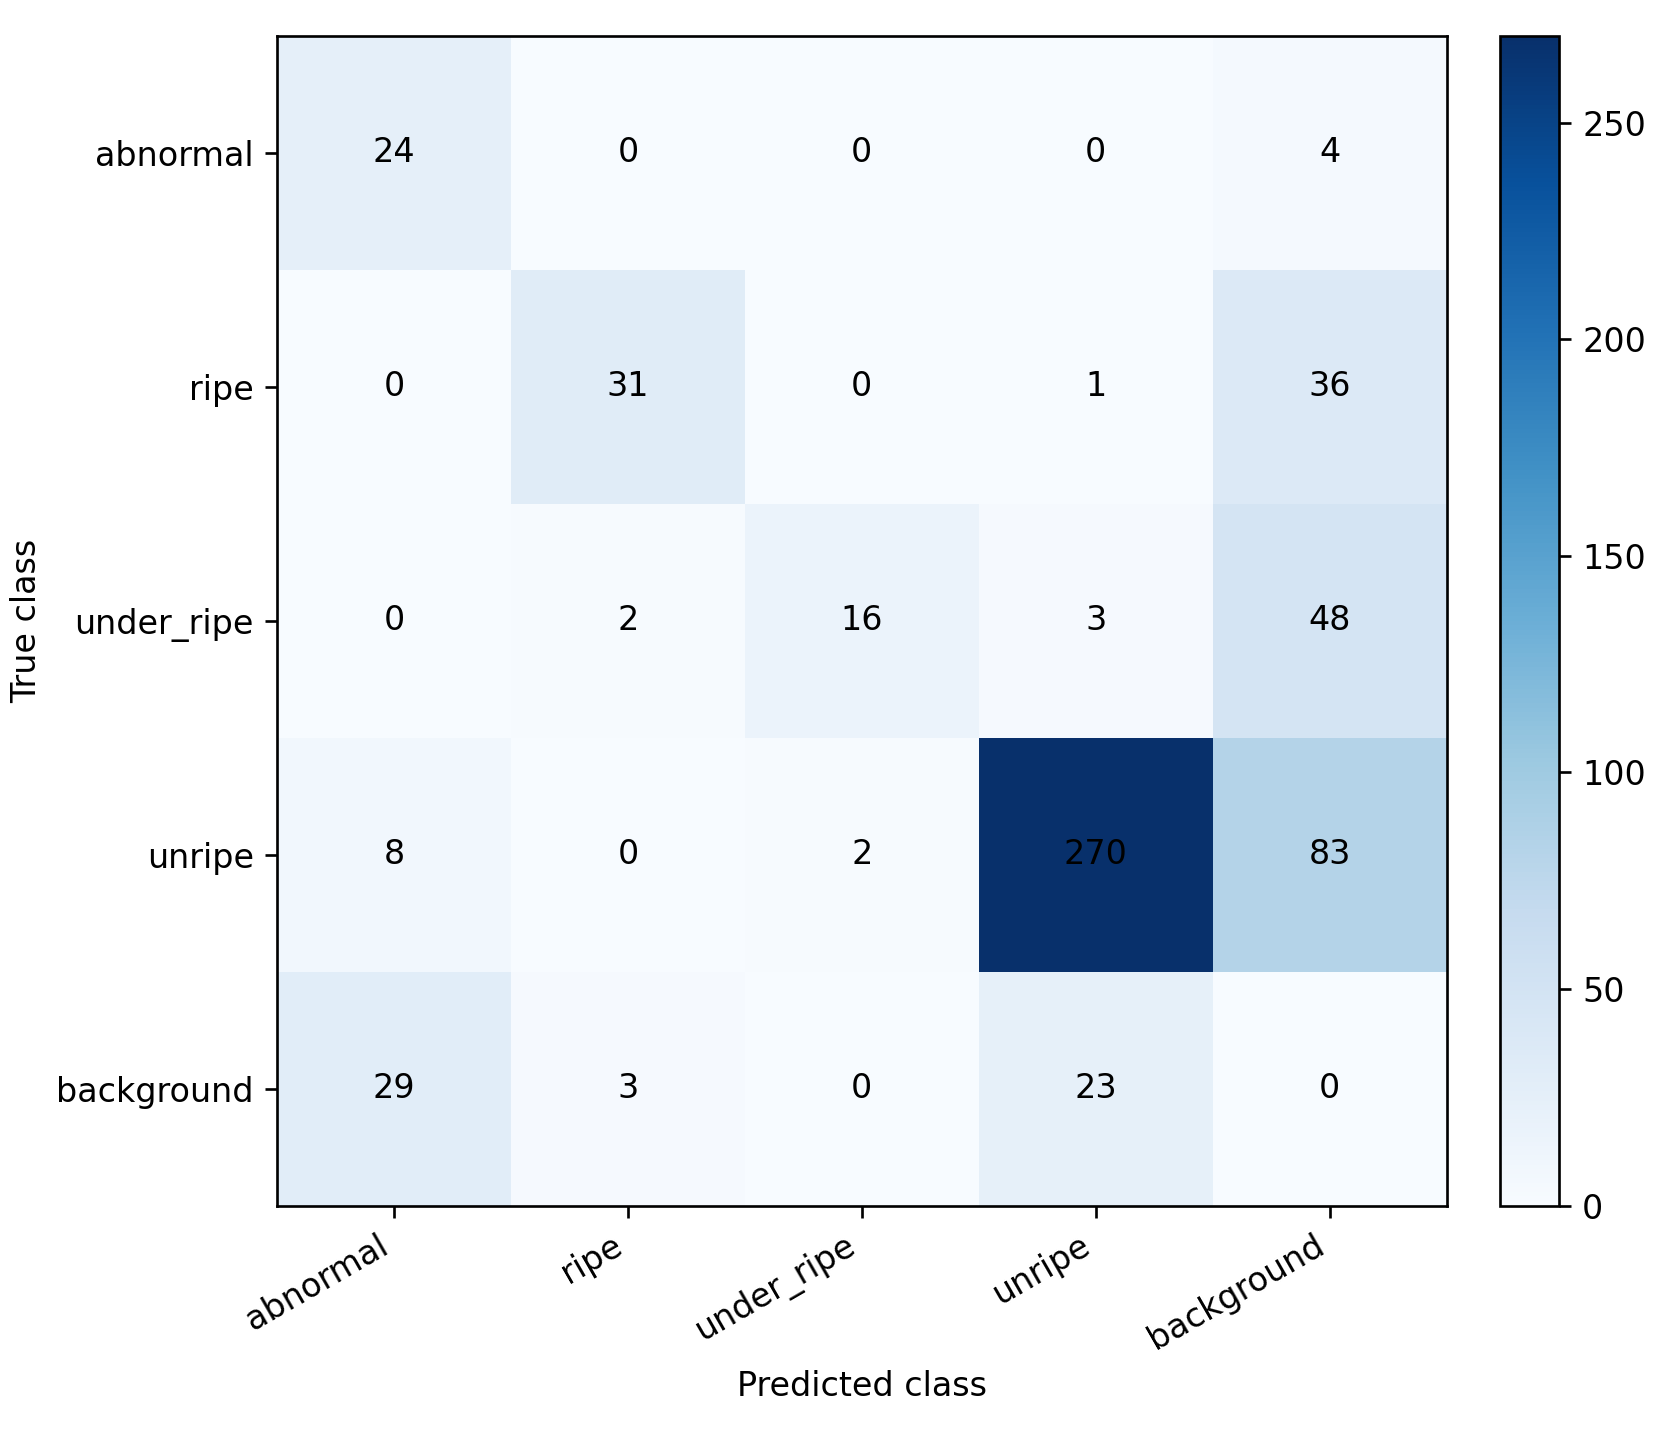
\includegraphics[width=0.75\textwidth]{figures/fig_strict_confusion_matrix.png}
\caption{Locked external-domain confusion matrix for the strict SSOD model under the four-class masked protocol.}
\label{fig:confusion_strict}
\end{figure}

\end{document}

